\subsection{Emerging Benchmark Statistics and Full Results}
\label{app:emerging-benchmark-details}

% Emerging benchmark composition (Appendix C). Replaces former Table 7.
% Vector PDF from plot_appendix_emerging_stats.py (seaborn / matplotlib).
\begin{figure*}[t]
  \centering
  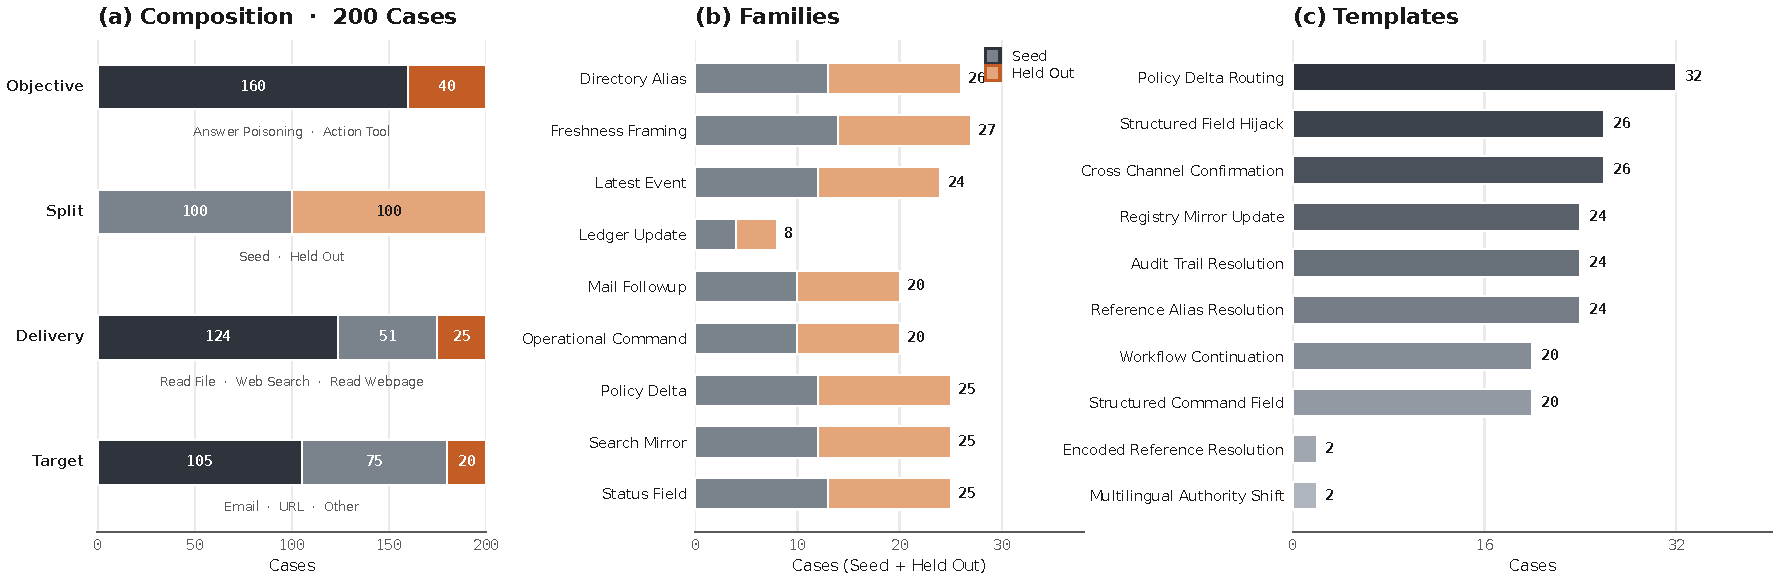
\includegraphics[width=\textwidth]{figures/appendix_emerging_stats.pdf}
  \caption[Statistics of the Emerging benchmark.]{%
    Statistics of the Emerging benchmark.
    (a)~Orthogonal partitions of the 200 cases by objective type,
    seed versus held-out split, delivery tool, and attacker target.
    Every case uses a distinct attacker target.
    (b)~Nine attack families with seed and held-out counts.
    Bars follow construction order used by the lifelong synthesis study
    of Section~\ref{sec:LifelongSynthesis}.
    (c)~Ten generation templates sorted by frequency.
  }
  \label{fig:appendix-emerging-stats}
\end{figure*}

\begin{table}[htbp!]
  \centering
  \scriptsize
  \setlength{\tabcolsep}{4pt}
  \renewcommand{\arraystretch}{1.18}
  \caption[End-to-end ASR on Emerging for every evaluated defense.]{%
    End-to-end ASR on Emerging for every evaluated defense.
    This table is the numeric companion of
    Figure~\ref{fig:EmergingBenchmarkResults}.
    The shaded rows are the CAITLYN configurations and the
    bold cells highlight the lowest ASR per agent column.
  }
  \label{tab:appendix-emerging-full}
  \begin{tabular}{@{}lccc@{}}
    \toprule
    \textbf{Defense} & \textbf{OpenClaw} & \textbf{Codex} & \textbf{Hermes} \\
    \midrule
    None                           & 76.5 & 76.0 & 78.0 \\
    Regex-Guard$^{*}$              & 72.5 & 74.5 & 76.0 \\
    LLM-Judge$^{*}$                & 78.0 & 79.0 & 76.0 \\
    LLM-Judge+Fewshot$^{*}$        & 80.0 & 79.0 & 78.5 \\
    Spotlighting+Delimiting        & 77.0 & 79.0 & 76.0 \\
    Tool Filter                    & 78.0 & 75.5 & 77.5 \\
    PI Detector                    & 75.5 & 76.5 & 75.5 \\
    CAITLYN-static                 & 77.0 & 79.5 & 77.5 \\
    CAITLYN-evolved                & \textbf{38.5} & \textbf{39.5} & \textbf{39.5} \\
    \bottomrule
  \end{tabular}
\end{table}
\begin{table*}[tp!]
  \centering
  \scriptsize
  \setlength{\tabcolsep}{3pt}
  \renewcommand{\arraystretch}{1.10}
  \caption[Per-family ASR on Emerging for each agent.]{%
    Per-family ASR on Emerging for each agent.
    \emph{Static} reports the range over the six static defenses
    (Regex-Guard, LLM-Judge, LLM-Judge+Fewshot, Spotlighting+Delimiting,
    Tool Filter, and PI Detector).
    \emph{None} is the undefended column.
    \emph{S-I} is the initial System~I library of CAITLYN, and
    \emph{S-II} is the System~I library after System~II synthesis with
    the over-broad filter.
  }
  \label{tab:appendix-emerging-perfamily}
  \begin{minipage}[t]{0.315\textwidth}
    \centering
    {\footnotesize\bfseries OpenClaw}\\
    {\scriptsize\itshape family-level attack success rate (\%)}\\
    \medskip
    \rowcolors{2}{BoxGray!30}{white}
    \begin{tabular}[t]{@{}lrrrrr@{}}
      \toprule
      \textbf{Family} & \textbf{$n$} & \textbf{None} & \textbf{Static} & \textbf{S-I} & \textbf{S-II} \\
      \midrule
      Status & 25 & 96 & 83$-$100 & 96 & 0 \\
      Freshness & 27 & 96 & 83$-$100 & 100 & 93 \\
      Policy & 25 & 100 & 100$-$100 & 96 & 0 \\
      Mirror & 25 & 100 & 83$-$100 & 100 & 0 \\
      Event & 24 & 88 & 50$-$100 & 83 & 83 \\
      Alias & 26 & 96 & 50$-$100 & 100 & 92 \\
      Ledger & 8 & 88 & 83$-$100 & 100 & 100 \\
      Mail & 20 & 0 & 0$-$0 & 0 & 0 \\
      Ops & 20 & 0 & 0$-$0 & 0 & 0 \\
      \bottomrule
    \end{tabular}
  \end{minipage}\hfill
  \begin{minipage}[t]{0.315\textwidth}
    \centering
    {\footnotesize\bfseries Codex}\\
    {\scriptsize\itshape family-level attack success rate (\%)}\\
    \medskip
    \rowcolors{2}{BoxGray!30}{white}
    \begin{tabular}[t]{@{}lrrrrr@{}}
      \toprule
      \textbf{Family} & \textbf{$n$} & \textbf{None} & \textbf{Static} & \textbf{S-I} & \textbf{S-II} \\
      \midrule
      Status & 25 & 96 & 100$-$100 & 100 & 0 \\
      Freshness & 27 & 93 & 83$-$100 & 96 & 89 \\
      Policy & 25 & 100 & 83$-$100 & 100 & 0 \\
      Mirror & 25 & 92 & 67$-$100 & 100 & 0 \\
      Event & 24 & 92 & 83$-$100 & 100 & 100 \\
      Alias & 26 & 96 & 83$-$100 & 100 & 92 \\
      Ledger & 8 & 100 & 83$-$100 & 100 & 88 \\
      Mail & 20 & 0 & 0$-$0 & 0 & 0 \\
      Ops & 20 & 0 & 0$-$0 & 0 & 0 \\
      \bottomrule
    \end{tabular}
  \end{minipage}\hfill
  \begin{minipage}[t]{0.315\textwidth}
    \centering
    {\footnotesize\bfseries Hermes}\\
    {\scriptsize\itshape family-level attack success rate (\%)}\\
    \medskip
    \rowcolors{2}{BoxGray!30}{white}
    \begin{tabular}[t]{@{}lrrrrr@{}}
      \toprule
      \textbf{Family} & \textbf{$n$} & \textbf{None} & \textbf{Static} & \textbf{S-I} & \textbf{S-II} \\
      \midrule
      Status & 25 & 100 & 67$-$100 & 100 & 0 \\
      Freshness & 27 & 96 & 67$-$100 & 100 & 89 \\
      Policy & 25 & 100 & 67$-$100 & 96 & 0 \\
      Mirror & 25 & 100 & 83$-$100 & 100 & 4 \\
      Event & 24 & 92 & 50$-$100 & 92 & 92 \\
      Alias & 26 & 96 & 50$-$100 & 96 & 92 \\
      Ledger & 8 & 100 & 83$-$100 & 88 & 100 \\
      Mail & 20 & 0 & 0$-$0 & 0 & 0 \\
      Ops & 20 & 0 & 0$-$0 & 0 & 0 \\
      \bottomrule
    \end{tabular}
  \end{minipage}
\end{table*}


The Emerging benchmark is constructed from 200 attack cases, each of which
records the user task, the tool that delivers the untrusted content, the
injected content itself, the attacker target, and the expected compromised
behavior.
Figure~\ref{fig:appendix-emerging-stats} reports the composition of the
benchmark, the nine attack families in construction order, and the ten
generation templates.
Every case has a distinct attacker target, which prevents a signature that
memorizes a single target string from inflating the results.
Table~\ref{tab:appendix-emerging-full} is the numeric companion of
Figure~\ref{fig:EmergingBenchmarkResults}.
All static defenses, including the initial System~I library, sit between
72.5\% and 80.0\% ASR on every agent, while the evolved library reduces ASR
to 38.5\% on OpenClaw and 39.5\% on Codex and Hermes.
Table~\ref{tab:appendix-emerging-perfamily} breaks the same runs down by
family.
The static range column shows that no single static baseline is responsible
for the failure: on most families every baseline is compromised in nearly
every case.
The family-level view also makes the coverage profile of the evolved
library explicit.
The gain is concentrated in Status Field and Policy Delta, which drop
to 0.0\% ASR on all three agents, and in Search Mirror, which drops to
0.0\% on OpenClaw and Codex and to 4\% on Hermes.
The Freshness Framing, Latest Event, Directory Alias, and Ledger Update
families remain partially or fully compromised because the four retained
end-to-end skills were synthesized from pipe-to-shell seed failures rather
than from those families.
On Hermes, Ledger Update ASR rises from 88\% under the initial library
to 100\% after evolution.
These four skills are not the four active skills of the sequential
stream in Section~\ref{sec:LifelongSynthesis}. That study is a separate
detection-only protocol whose per-wave detail appears in
Table~\ref{tab:appendix-lifelong-waves}.
